\documentclass[man]{apa2}
\usepackage{pslatex}
\usepackage{amssymb}
\usepackage{graphicx}
\usepackage{color}
\usepackage{covington}
\usepackage[usenames,dvipsnames]{xcolor}

\title{Young children's developing sensitivity to discourse continuity as a cue for inferring reference}

\twoauthors{Alexandra C. Horowitz}{Michael C. Frank}
\twoaffiliations{Department of Psychology, Stanford University}{Department of Psychology, Stanford University}


\abstract{Children encounter many opportunities for word learning where a novel word (e.g., ``chinchilla'') coincides in time with the presence of its referent (e.g., a parent pointing at a fuzzy rodent). These two ingredients are not always present simultaneously, however, but they sometimes still occur in succession within a discourse.  We investigated children's ability to apply their knowledge of discourse structure to infer the referent of a novel word in the absence of social cues like pointing or eye-gaze.  In Experiment 1A, we introduced 2- to 6-year-old children and adults to two novel toys, and described each using two sentences.  We embedded the introduction of a novel label (``Have you seen a toma before?'') between the two sentences about one of the toys, with no cues giving the label's referent other that its position in the discourse. Adults and children older than three were more likely to attribute the label to the toy whose descriptions surrounded the naming event. In Experiment 1B, we tested whether participants made their selections based on temporal associations---choosing the toy that was described closest in time to the naming event---rather than inferences about discourse. Participants heard the novel label introduced after the two descriptions of a toy rather than embedded between them. Both children and adults responded close to chance in this experiment, indicating that temporal proximity alone did not guide their selections. Together, these results suggest that children can use discourse position to make inferences about reference in word learning situations.

~\\

Keywords: discourse; disambiguation; language development; pragmatics}

\shorttitle{Discourse as a Cue for Inferring Reference}
\rightheader{Discourse as a Cue for Inferring Reference}

\acknowledgements{Special thanks to the staff and families at the San Jose Children's Discovery Museum. This work supported by a John Merck Scholars Fellowship to MCF. An earlier version of this work was presented to the Cognitive Science Society in \citeA{horowitz2013}.

~\\

\noindent Address all correspondence to Alexandra C. Horowitz, Stanford University, Department of Psychology, Jordan Hall, 450 Serra Mall (Bldg. 420), Stanford, CA, 94305. Phone: 650-721-9270. E-mail: \texttt{ahorowit@stanford.edu}}

\begin{document}

\maketitle                            


\section{Introduction}

Children can use many strategies to learn new words.  In overtly pedagogical situations, adults employ cues like pointing and other signals of joint attention to establish reference and help children to learn word meanings \cite{bakeman1984,csibra2010,hollich2000}.  Unambiguous ostensive cues are not available at all times, however.  If children are to learn in more ambiguous situations, they must rely on other strategies to infer the meanings of novel words. Here we consider discourse structure---the order of utterances and how they relate to each other---as a cue. We focus particularly on \emph{discourse continuity}, the idea that sentences in close succession are more likely to relate to the same topic. The current study measures children's ability to use discourse continuity to make inferences about the referent of novel words in simple, grounded contexts.

Children are exposed to information about discourse structure whenever they hear speech, and the simple linking of topics across sentences could provide a valuable source of information about the meanings of words. From an utterance such as,

\begin{example}
\label{ex:chin1}
I love chinchillas!
\end{example}

\noindent a child may not be able to infer what ``chinchilla'' means. But consider this same utterance as embedded in a short discourse:

\begin{example}
\label{ex:chin2}
I got a new pet. \\ I love chinchillas! \\ They're so soft.
\end{example}

\noindent The discourse structure in Example (\ref{ex:chin2}) might allow a child to make inferences that (A) a chinchilla is a kind of animal, and (B) chinchillas are probably furry.  The linking of information across a sequence of utterances requires that children have some understanding of discourse structure.  For inference (A), the child must assume that the statement in the second utterance is topically related to the first, and for inference (B), the child must assume that the pronoun in the third co-refers to the noun in the second. 

We focus here on inferences like (A). We begin by discussing adults' recognition of discourse structure cues and how these abilities may relate to children's language processing; we then discuss links between these abilities and word learning. Our review of previous literature sets the stage for our experiment, which tests whether adults and children are able to make a simplified version of this inference, using an assumption of discourse continuity to infer which object is referred to by a novel term.
 
Throughout this discussion, the perspective we take on word learning is that there are (at least) two problems that learners jointly solve \cite{frank2009,mcmurray2012}: first, the problem of in-the-moment referential ambiguity, and second, the longer-term problem of finding the conceptual extension of a word (even when its referent is known). We refer to the first problem as the problem of determining reference, and the second problem as the generalization problem. Although (2) highlights the potential of discourse information for both problems, here we focus on the role of discourse in referent selection.\footnote{A somewhat orthogonal concern about calling this type of example word learning has to do with children's retention of the referents they select. Some recent work indicates that although young children can use in-the-moment information to make inferences about reference, mappings inferred in this way are not necessarily retained \cite{horst2008,bion2012}. Our current work does not address long-term word learning, but instead focuses on investigating children's in-the-moment inferences about reference.}

\subsection{Discourse Structure and Referent Selection}

Discourse in adult speech is often structured around the introduction and subsequent discussion of particular topics \cite<e.g.>{ariel1990,clark1996,gundel1993,prince1992}. The first mention of a new topic or entity tends to be used to establish reference: it is usually longer and more explicit than subsequent mentions. These later mentions (when the topic is ``given'') presuppose that the topic under discussion is in common ground and tend refer back to it with elaborations, often reducing the reference to a pronoun or a shortened name. Linguists and computational linguists have explored a number of proposals for capturing the complex structures that appear in spoken and written discourses between adults \cite{asher2003,grosz1995,hobbs1979,kehler2002,mann1988,polanyi1988,wolf2005}. In the current context, we will focus on a simpler operationalization of discourse as repeated mentions of the same referent \cite{frank2013,rohde2014}.

Some recent observational work suggests a possible role for discourse continuity in word learning. \citeA{frank2013} examined a video corpus of caregivers interacting with their 6- to 18-month-old children around pairs of toys. For each utterance, they annotated what object the parent was looking at, pointing to, and talking about, and found that the referent of the parent's previous utterance was as strong a cue to the referent of the current utterance as was any individual social cue (e.g. pointing or the parent's gaze). In other words, a child trying to guess the topic of the sentence would do well to assume continuity of reference between utterances to ``smooth'' the input from noisy and often irregularly-used social cues.

In addition, other social and linguistic factors may mark discourse in child-directed speech. A followup to this first observational study tested whether findings on discourse structure in adults would generalize to child-directed speech \cite{rohde2014}. This study found that both the social cues that accompanied object references and the form of these references changed over the course of a topical discourse. Early on in the discourse, an object referent was more likely to be highlighted with social cues and referred to at the end of an utterance. In contrast, later references were less likely to be highlighted, were more pronominal, and were less likely to be in final (``topic'') position in the utterance. 

Complementing observational data that signal the presence of discourse information in child-directed speech, children also show sensitivity to conventions of continued reference within a discourse structure by 2 -- 3 years of age.  They are quite effective in tracking the shift from new to given in communications about grounded referents, and in their own productions, their reference conventions and their choices of which labels to omit both show sensitivity to these features \cite{allen2000, bates1976, greenfield1976, clancy2004, skarabela2007}.  Children also seem to be able to use the typical position of a first mention (at the end of an utterance, in ``topic position'') to infer the referent of an ambiguous pronoun \cite{song2005, song2007, pyykkonen2010}, although evidence is somewhat mixed on this question \cite{arnold2007}. This body of work as a whole suggests that children's production and comprehension shows substantial evidence of understanding basic discourse structure, though no studies to our knowledge link this knowledge to word learning specifically.

Nevertheless, there is a substantial body of work suggesting that children can incorporate speakers' social and pragmatic cues within a discourse to infer the intended referent of novel words. By 18 months old, toddlers map novel labels to novel objects that the speaker attends to rather than what they themselves may be attending to, even after a time delay \cite{baldwin1991,baldwin1993}.  Young children apply new terms to the target of a speaker's search \cite{tomasello1994} and appear to be able to track whether experiences have been shared with a partner to map a speaker's introduction of new information to what is novel to that speaker (\citeNP{akhtar1996}, but see \citeNP{samuelson1998}; we discuss these studies in greater depth in the General Discussion).  All of these findings suggest that children make inferences about the referents for novel words by assuming that speakers are using language to communicate about their own focus of attention.  The evidence thus supports the conclusion that young children can integrate available discourse and social cues to infer meaning. It is still unclear, however, whether they rely on social information to disambiguate reference, or whether they can make inferences about intended meaning from discourses cues alone. 

\subsection{The Current Study}

The proposal that emerged from the \citeA{frank2013} and \citeA{rohde2014} studies was the assumption that ongoing topic information through discourse continuity might help children to connect social cues with labels, even if the labels and cues do not co-occur in a single utterance.  For example, consider the following (invented) utterance pair:
%that occurred in utterances either before or after. 

\begin{example}
\label{ex:blicket}
Look at this! [speaker momentarily points at toy] \\
This one is a blicket.
\end{example}

\noindent Despite how obvious the pairing is between the two utterances, some sort of inference about continued reference in discourse (such as the ones described in Example \ref{ex:chin2}) would still be necessary to lead a child to believe that the toy that was pointed to is a blicket.  Although the observational data suggested this kind of inference as a possible mechanism for applying discourse structure to help in word learning, Frank et al.'s findings provided no evidence that children in the study actually could use this mechanism.  The goal of our current study is to provide a test of this proposal. 

We discuss two experiments investigating children's and adults' sensitivity to discourse continuity to resolve reference ambiguity (and hence facilitate inferences about word meaning). In Experiment 1A, we show that children and adults can infer word meaning from sequentially offset social cues (as in Example \ref{ex:blicket}), using information about discourse continuity.  In Experiment 1B, we show that the results from Experiment 1A are not due to participants relying solely on temporal proximity to resolve ambiguity.  Together, our findings suggest that language users are able to apply their knowledge about how utterances relate within a discourse to make inferences about speakers' intended referents.  Overall, this work suggests that children are not constrained to use social and contextual cues from individual utterances alone, but can evaluate how information may relate across broader discourses and can use this information to infer word meanings.

\section{Experiment 1A}

We designed an experimental task to investigate children's recognition of discourse structure as a cue to reference. We created trials with two minimal discourse topics, each consisting of two grouped sentences describing a single toy.  We then introduced participants (children ages 2 -- 6 years and a comparison group of adults) to two novel toys at a time, accompanied by only one novel label.  We manipulated where in discourse the name was introduced, critically presenting the new label between the two descriptions of either the First Toy or the Second Toy.  We call this an \emph{Embedded} label because the introduction of the name is embedded between two descriptions of the same toy, thus embedded within a topic.  This design is pictured in Figure \ref{fig:demo}.

We were interested in which toy participants selected as the referent of the label.  We predicted that, if listeners were sensitive to how information relates within discourse structure, then they would be more likely to select the toy whose descriptions surrounded the naming event.  Critically, because the experimenter made eye contact with the participant during the actual naming event and gave no gaze or gesture cues to the referent of the label, the only cue to the novel word's reference was the location in which the name was introduced within the broader discourse.  This design allowed us to examine listeners' use of discourse information to resolve local referential ambiguity.  


\begin{figure} 
  \begin{center} 
    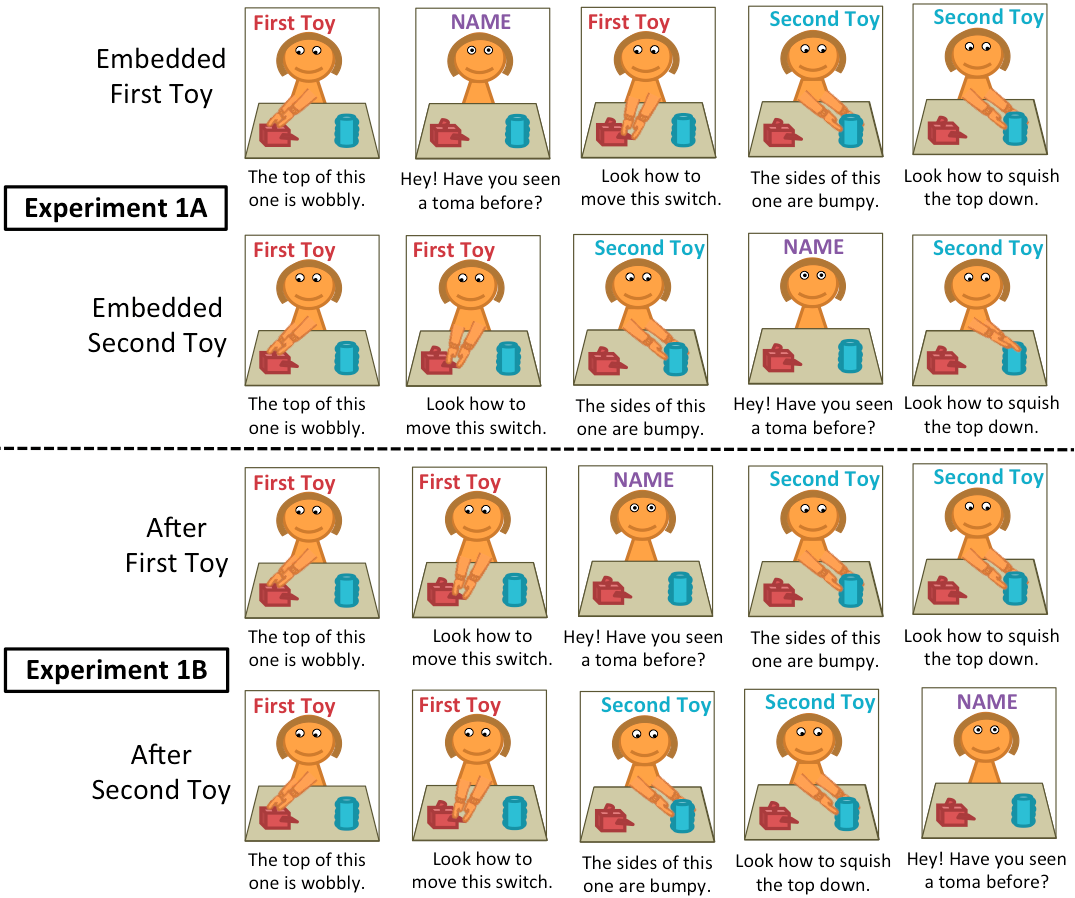
\includegraphics[width=6in]{figures/continuity_demo_all_trials.png} 
    \caption{\label{fig:demo} Schematic order of events for ``Second Toy'' trials across Experiments (``First Toy" trials not pictured). In Experiment 1A (\emph{Embedded} trials), the experimenter made eye contact without other gaze cues and introduced the naming event between two descriptions of a single toy.  In Experiment 1B (\emph{After} trials), events were identical except that the experimenter introduced the naming event after two descriptions of a toy.} 
  \end{center} 
\end{figure}	

\section{Methods}


\subsection{Participants}

A planned sample of 64 children was recruited from the San Jose Children's Discovery Museum.  Participants were uniquely identified by their birth dates to prevent repeat inclusion in the study.  Children were given a sticker and certificate as compensation their participation.  Parents were asked to fill out a short demographic form about their children's language background, and only children who were reported to hear English at least 75\% of the time were included in the study.  Seven additional children were recruited but excluded for not meeting this criterion: three children due to insufficient English exposure and four children whose language information was not reported.\footnote{As part of our partnership with Children's Discovery Museum, we invite any interested visitors to participate in our studies rather than prescreening children to meet our language requirements \cite{callanan2012}. This standard to recruit inclusively also accounts for variability in gender counts across conditions.}

Children were recruited in four age groups: 2-year-olds (n = 16, 12 girls, mean age 2 years 7 months), 3-year-olds (n = 16, 4 girls, mean age 3 years 6 months), 4-year-olds (n = 16, 6 girls, mean age 4 years 5 months), and 5-year-olds (n = 16, 8 girls, mean age 5 years 4 months).  

We also recruited a comparison group of twelve adults from the museum, none of whom had children who participated in the study. Adults filled out a brief demographic form reporting their own language background, and only adults using English at least 75\% of the time were included in the final sample. Only one additional participant was excluded for reporting less than this amount of English use.  


\subsection{Stimuli}

Four pairs of unusual items (e.g. a faucet aerator and a spaghetti measure) served as the novel toys.  An additional item (an oddly-shaped funnel) was used for training. Pictures of all toys are given in Appendix A.

\subsection{Procedure}

Participants were seated across from the experimenter in a quiet room at the museum.  Children participated in a training trial featuring ostensive labeling of a single toy (``This toy is called a blicket.  Can you point to the blicket?'') to familiarize them to the design and to practice pointing before seeing four discourse disambiguation trials.  Adults participated in the four discourse disambiguation trials without undergoing the initial training. 

For the discourse disambiguation trials, the experimenter placed a unique set of two toys on the table and described each in turn (see Figure \ref{fig:demo}, top).  In these Embedded trials, the experimenter introduced the naming event between two sentences about the same toy.  The labels introduced in the four trials were ``toma,'' ``modi,'' ``gazzer,'' and ``zib.''  Each participant heard a naming event embedded between descriptions of the first toy for two of the trials (``First Toy'' trials) and between descriptions of the second toy for two of the trials (``Second Toy'' trials).  Label location, trial order, toy pairs, and target side were counterbalanced across participants.  

When describing the toys, the experimenter directed her gaze to the toy and demonstrated a feature of the toy.  There was a brief pause between each sentence.  For the naming event, she disengaged from the toy and maintained a neutral position while drawing participants' attention by using their names and establishing eye contact.  The experimenter did not give any gaze cues or other indicators to the referent of the novel name.  Thus, the naming event in itself carried no information to guide disambiguation; the only cue available was its location within discourse.  The toy pair remained in view of participants throughout the duration of the trial.  At the end of each trial, the experimenter prompted participants to identify the named item by pointing (e.g. ``Can you point to the toma? Which one is the toma?'').  If children did not respond immediately, they were prompted again to make their best guess. The sessions were videotaped and coded offline. The entire task took about 5 minutes to complete. 
 

\subsection{Results}

Despite the lack of coincident social cues to disambiguate the label, older children and adults were both overall much more likely to select the toy whose descriptions surrounded the naming event, suggesting that they can recognize and make inferences from discourse continuity.  Figure \ref{fig:res5}, left, illustrates the proportion of children and adults selecting the second toy as the referent of the label across trial types (whether the label was introduced with the First Toy or the Second Toy). Three-year-olds' responses appeared to be sensitive to naming condition, and five-year-olds' ability to use topic continuity in this paradigm was comparable to adult performance.


\begin{figure}
  \begin{center} 
    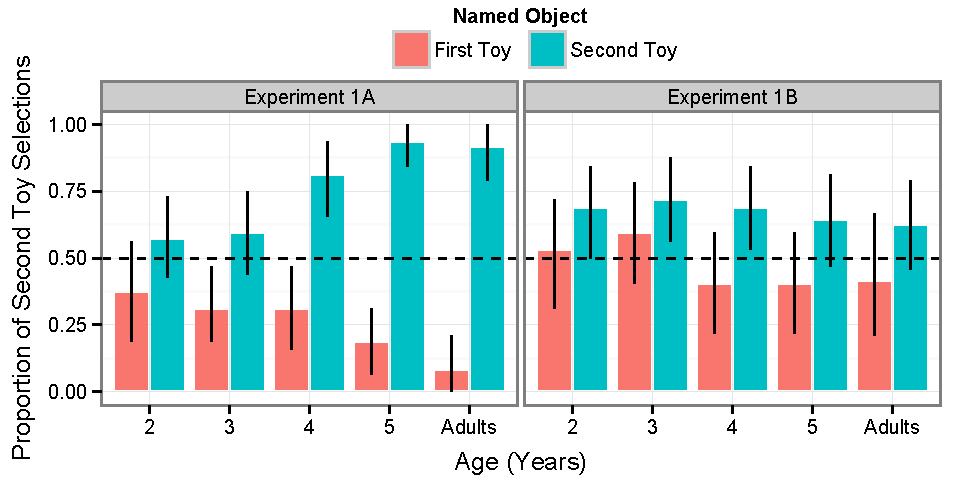
\includegraphics[width=6in]{figures/continuity_kids_and_adults_barplot_mod.pdf} 
    \caption{\label{fig:res5} Combined data from Experiments 1A and 1B.  Mean proportion of selection of the second toy across Experiment (\emph{Embedded} or \emph{After}) and trial type (label given with First Toy or Second Toy), plotted by age group. The dashed line indicates chance performance, and error bars show 95\% confidence intervals, computed by a non-parametric bootstrap over participants.} 
  \end{center} 
\end{figure}	



  \begin{table} [t]
   \caption{Coefficient estimates from generalized linear mixed models predicting toy selection as an interaction between trial type and age with random effects of participant and trial type for Experiment 1A (left) and Experiment 1B (right).
   \label{tab:coefficient_estimates} } 
   \begin{center} 
     \begin{tabular}{lrrrr|rrrr} 
          & \multicolumn{4}{c}{Experiment 1A: Embedded trials} &  \multicolumn{4}{c}{Experiment 1B: After trials}\\
                      \hline 
       \null  & Coef. & Std. Err. & $z$  &  $p(|z|)$ & Coef. & Std. Err. & $z$  &  $p(|z|)$  \\ 
       \hline  
        Age   & -0.27 	&  0.20 & -1.40 & 0.16						               & -0.21 & 0.21 & -0.98 & 0.40\\ 
        Trial type   & -2.24 & 1.17 &  -1.92 & 0.06				                       & 0.00 & 1.13 & 0.00 & 0.99 \\
        Age $\times$ Trial type    & 1.10 & 0.30 & 3.61 &\textbf{ $<$0.001} 		& 0.23 & 0.27 & 0.83 & 0.41\\ 
       \hline 
     \end{tabular} 
  \end{center}
 \end{table}
 

To measure the reliability of these patterns, we fit a generalized linear mixed effects model predicting second toy selection as an interaction between trial type (naming event with the First Toy or Second Toy) and age, with random effects of participant and trial type (the maximal structure appropriate for our experimental design; \citeNP{barr2013}). Age was treated as a continuous variable. This model found no main effect of age and a trend towards a main effect of trial type, indicating that children and adults were overall somewhat more likely to select the second toy in Second Toy trials. The primary effect, however, was a significant interaction between age and trial type, indicating that participants' reference selections by naming location increased with age. Coefficient estimates from these models are shown in Table \ref{tab:coefficient_estimates}, left.

%This model found significant differences in toy selection by both trial type and age group, such by 4-year-olds exhibited marginally stronger performance than 2-year-olds at selecting the toy according to the embedded naming location. Five-year-olds and adults were significantly more likely to show this response pattern. 

%    agegroup condition   correct        sd
% 1         2     After 0.5781250 0.1983001
% 2         3     After 0.5625000 0.2661453
% 3         4     After 0.6406250 0.2882237
% 4         5     After 0.6250000 0.2886751
% 5     adult     After 0.6041667 0.3100281
% 6         2    During 0.6093750 0.3158157
% 7         3    During 0.6406250 0.2230237
% 8         4    During 0.7500000 0.1825742
% 9         5    During 0.8750000 0.1825742
% 10    adult    During 0.9166667 0.1230915

  \begin{table} [t]
  \caption{Mean proportion correct and standard deviation for participants' selection of the toy matching the naming location across trial types, as well as results from paired $t$-tests examining response differences across trial types (naming location with the First Toy or Second Toy). Proportions were computed as the proportion choosing the first toy in a First Toy trial and proportion choosing the second toy in a Second Toy trial.\label{tab:2} } 
  \begin{center} 
    \begin{tabular}{lccrrr|ccrrr} 
         & \multicolumn{5}{c}{Experiment 1A: {\it Embedded} trials} &  \multicolumn{5}{c}{Experiment 1B: {\it After} trials}\\
                     \hline 
      \null Age & Prop. & SD & $t$-value & df & $p$-value  & Prop. & SD & $t$-value & df & $p$-value  \\ 
      \hline  
       2--3  & 0.61 & 0.32 & -1.23 & 15 & 0.24                          & 0.58 & 0.20 & -1.58 & 15& 0.14\\ 
       3--4  & 0.65 & 0.22 & -2.52 & 15 & \textbf{0.02}            & 0.56 & 0.27 & -.94 & 15 & 0.36 \\ 
       4--5  & 0.75 & 0.18 & -5.48 & 15 & \textbf{$<$0.01}     & 0.64 & 0.29 &-1.95 & 15 & 0.07\\
       5--6  & 0.88 & 0.18 & -8.22 & 15 & \textbf{$<$0.01}      & 0.63 & 0.29  & -1.62 & 15 & 0.13\\ 
       Adults & 0.92 & 0.12 & -11.73 & 11 & \textbf{$<$0.001} & 0.60 & 0.31 & -1.16 & 11 & 0.27 \\
      \hline 
    \end{tabular} 
 \end{center}
\end{table}

We also ran a series of paired $t$-tests to examine response differences between trial types for each age group (Table \ref{tab:2}, left).  Significant differences in reference selection were found across First Toy and Second Toy Embedded trial types for children ages 3 -- 6 years.

Our results in Experiment 1A suggest that listeners are sensitive to discourse continuity to resolve reference ambiguity.  By varying where a novel label was embedded within a topic, we found that older children and adults systematically selected the toy whose descriptions bracketed the naming event, suggesting that they were sensitive to where in the discourse the name was introduced.  However, it is possible that listeners were using other heuristics to make their selections rather than relying on the discourse structure per se \cite{samuelson1998}.  In order to investigate this possibility, we ran a second experiment to dissociate discourse continuity from simpler associative strategies. 

% DURING
% (Intercept)      0.1500     0.7835   0.191 0.848135    
% age             -0.2737     0.1963  -1.395 0.163161    
% corr.sideB      -2.2434     1.1703  -1.917 0.055241 .  
% age:corr.sideB   1.0995     0.3049   3.606 0.000311 ***

% AFTER
%                  Estimate Std. Error z value Pr(>|z|)
% (Intercept)     0.7366232  0.8800883   0.837    0.403
% age            -0.2097612  0.2135395  -0.982    0.326
% corr.sideB      0.0008899  1.1286078   0.001    0.999
% age:corr.sideB  0.2266775  0.2734905   0.829    0.407

 
 
\section{Experiment 1B}

Experiment 1A showed that children and adults chose the toy whose descriptions surrounded the naming events. A high-level explanation for this finding is that listeners assumed that these sentences formed part of a broader discourse about the toy. Nevertheless, the data are also consistent with a lower-level explanation: Participants could be making a temporal association between the label and the toy descriptions, rather than necessarily considering discourse structure. That is, participants could have been selecting the toy that was described nearest to the naming event in time, which in Experiment 1A would always correspond with the toy surrounding the introduction of the label in Embedded trials. 

Experiment 1B was designed to rule out this particular version of a temporal proximity hypothesis.  We made a slight modification to the scripts such that the naming event was moved to be introduced \emph{after} descriptions of either the First Toy or the Second Toy rather than embedded between descriptions of that toy.  
Thus in these \emph{After} trials, the naming event could occur next to descriptions of both toys in ``After First Toy'' trials, or next to only the second toy in ``After Second Toy'' trials. As before, a schematic of our design is shown in Figure \ref{fig:demo}.

This design allowed us to make the following predictions:  If children relied on temporal association as a heuristic, they would be at chance in the After First Toy trials (where the label can refer to either one or the other toy).  In the After Second Toy trials, however, they would systematically select the second toy (because this is the only item that receives any attention from the speaker proximate to the naming event). In contrast, if children's responses depended on discourse continuity information instead of temporal associations, then they would guess at chance in both trial types, because the naming event always occured \emph{after} the discussion of a topic rather than being embedded within the topic. 

\section{Methods}

\subsection{Participants}

A new planned sample of 64 children was recruited from the San Jose Children's Discovery Museum. As before, children were recruited in four age groups: 2-year-olds (n = 16, 6 girls, mean age 2 years 6 months), 3-year-olds  (n = 16, 6 girls, mean age 3 years 6 months), 4-year-olds (n = 16, 8 girls, mean age 4 years 6 months), and 5-year-olds (n = 16, 10 girls, mean age 5 years 5 months).  Five additional children were excluded due to insufficient English exposure, six children were excluded whose language information was not reported, and four children were excluded for not completing all four trials of the study.  Also as before, we recruited a group of twelve adults, all of whom reported using English at least 75\% of the time and had not seen the study before.  Birth dates and video records confirmed that none of our participants had taken part in Experiment 1A. 

\subsection{Stimuli}

Stimuli were identical to Experiment 1A. 

\subsection{Procedures}

Procedures were identical to Experiment 1A, with one minor change to the script of each trial: The location of the naming event was moved to occur after two descriptions of a toy rather than being embedded between the two descriptions. Thus, participants in Experiment 1B heard all of the same sentences and demonstrations as in Experiment 1A, the only difference was the discourse location where the label was introduced; for two trials the label was introduced after descriptions of the first toy (``After First Toy'' trials), and for two trials the label was introduced after descriptions of the second toy (``After Second Toy'' trials).  

\subsection{Results}

As predicted, children and adults were at chance in the After First Toy trials, and showed only a weak bias to use temporal proximity to disambiguate reference in After Second Toy trials. Figure \ref{fig:res5}, right, illustrates the proportion of children and adults selecting the second toy as the referent of the label by naming location.  Paired $t$-tests between reference selections across After First Toy and After Second Toy trials for each age group indicated that there were no significant differences in toy selection by trial type for any age group, though there was a trend towards such an effect in the 4-year-old group (Table \ref{tab:2}, right). 

% data:  subset(agg.data.s, agg.data.s$agegroup == "2" & condition ==     "After" & corr.side == "B")$side - 0.5
% t = 2.0868, df = 15, p-value = 0.05439

% data:  subset(agg.data.s, agg.data.s$agegroup == "3" & condition ==     "After" & corr.side == "B")$side - 0.5
% t = 2.7815, df = 15, p-value = 0.01397

% data:  subset(agg.data.s, agg.data.s$agegroup == "4" & condition ==     "After" & corr.side == "B")$side - 0.5
% t = 2.0868, df = 15, p-value = 0.05439

% data:  subset(agg.data.s, agg.data.s$agegroup == "5" & condition ==     "After" & corr.side == "B")$side - 0.5
% t = 1.6231, df = 15, p-value = 0.1254

% data:  subset(agg.data.s, agg.data.s$agegroup == "adult" & condition ==     "After" & corr.side == "B")$side - 0.5
% t = 1.3933, df = 11, p-value = 0.1911

Because predictions differed between After First Toy and After Second Toy trials, however, we also tested whether there was any temporal bias specifically in After Second Toy trials. We conducted one-sample $t$-tests between means from participants in each group and chance. These tests revealed a different developmental pattern from results in the pairwise tests (and from results in Experiment 1A). Performance was reliable or close to reliable for 2-, 3-, and 4-year-olds ($t(15) = 2.09$, $2.78$, and $2.09$, $p = .054$, $.01$, and $.054$ respectively). In contrast, performance for 5-year-olds and adults was not reliably different from chance ($t(15) = 1.62$ and $1.39$, $p = .13$ and $.19$, respectively). 

To analyze performance patterns across trial types, we fit a generalized linear mixed effects model as in Experiment 1A by predicting toy selection as an interaction between trial type and age with random effects of participant.  There were no significant effects in the model, indicating that---given the level of power achieved in this study---we could not measure reliable differences in response between After First Toy and After Second Toy trials. Coefficient estimates from the model are shown in Table \ref{tab:coefficient_estimates}, right. Taken together, our findings suggest that younger children might have been somewhat more likely than chance to rely on temporal association, but we cannot draw strong conclusions due to the lack of differences between First Toy and Second Toy trial types. 

% age                             -0.1834     0.1834  -1.000   0.3174  
% corr.sideB                       0.0582     1.0602   0.055   0.9562  
% conditionDuring                 -0.4841     1.1312  -0.428   0.6687  
% corr.sideB:age                   0.1999     0.2569   0.778   0.4364  
% conditionDuring:age             -0.1085     0.2795  -0.388   0.6979  
% conditionDuring:corr.sideB      -2.2733     1.5939  -1.426   0.1538  
% conditionDuring:corr.sideB:age   0.9033     0.4019   2.247   0.0246 *
  \begin{table} [t]
   \caption{Coefficient estimates from a generalized linear mixed models predicting toy selection as an interaction between trial type, age, and experiment.
   \label{tab:coefficient_estimates_full} } 
   \begin{center} 
     \begin{tabular}{lrrrr} 
       \hline 
       \null  & Coef. & Std. Err. & $z$  &  $p(|z|)$ \\
       \hline  
        Age                                                                     & -0.18 &  0.18 & -1.00 & 0.32 \\
        Trial type                                                            & 0.06 &1.06 &  0.06 & 0.96 \\
        Experiment                                                         & -0.48 & 1.13 &  -0.43 & 0.67 \\
        Age $\times$ Trial type                                      & 0.20 & 0.26 & 0.78 & 0.44\\ 
        Age $\times$ Experiment                                   & -0.11 & 0.28 & -0.39 & 0.70\\ 
        Trial type $\times$ Experiment                          & -2.27 & 1.59 & -1.43 & 0.15 \\ 
        Age $\times$ Trial type $\times$ Experiment    & 0.90 & 0.40 & 2.25 & {\bf 0.02} \\ 
       \hline 
     \end{tabular} 
  \end{center}
 \end{table}
 
To test whether participants' performance in Experiment 1A could reliably be distinguished from participants' performance in Experiment 1B, we additionally fit a combined generalized linear mixed effects model across the data from both experiments, adding experiment as an additional between-subjects factor (Table \ref{tab:coefficient_estimates_full}).  The only reliable effect in this model was a three-way interaction between experiment, trial type, and age, indicating that, with increasing age, children were more likely to select the first toy in First Toy trials and the second toy in Second Toy trials, for Experiment 1A more than Experiment 1B. This analysis confirms that the behavior and developmental trend we observed in Experiment 1A and attributed to use of discourse information was distinct (at least for older children) than the trends we observed in Experiment 1B and attributed to temporal association.

\section{General Discussion} 

We investigated whether adults and children could use position in discourse as a cue to connect social information with an ambiguous label. In our experiments, adults made effective use of discourse position and children showed increasing sensitivity to discourse position with age. In addition, all age groups except the 2-year-olds showed some evidence of using discourse position information. Taken together, our findings suggest a potential role for discourse continuity in helping children use communicative information in otherwise ambiguous contexts, and strengthen the argument that models of word learning should incorporate discourse information as a valuable cue to reference and perhaps meaning.

\subsection{Possible Alternative Accounts of Our Findings}

We discuss a number of alternative accounts of our finding in Experiment 1A. In particular, we address whether our results could have been due to the general temporal proximity of labels to referents, whether they could have been the result of a strategy of linking words to the most proximal previously-mentioned referent, or whether they could have been due to differences in the number of referential comments prior to the labeling event (``weighted proximity''). 

Could children have simply relied on temporal proximity to resolve local referential ambiguities? Our data clearly rule out this explanation. In particular, our After Second Toy trials in Experiment 1B presented only a single possible referent adjacent to the naming event.  Despite the temporal proximity of the second toy to the labeling event, children showed only a weak bias to choose it in these trials.  Additionally, this bias was stronger for younger children, in contrast to the stronger use of discourse information by older children.\footnote{In principle, one possible interpretation of the critical After Second Toy trials from Experiment 1B is that participants guessed that the label referred to both objects at once. In practice we did not hear any comments that suggested this in participants' responses. In addition, the toys were sufficiently dissimilar to make this explanation unlikely unless the experiment consisted of using many different superordinate synonyms for ``artifact'' or ``thing.''} Thus the data do not support a pure temporal proximity account.

Our results from the After trials rule out another possible account as well. According to this account, in the absence of social cues to meaning, children assume the speaker's use of a novel label serves the goal of referring to the item she was just discussing (a ``previous mention'' bias; similar to temporal proximity but unidirectional). Children's behavior in the Embedded trials was consistent with this account---in Embedded trials, the target toy was described immediately before the experimenter provided a novel label. But in After First Toy trials, a ``previous-mention'' account would have predicted an even stronger bias towards the first toy, which we did not observe.

% . A discourse-based variant of this explanation does seem potentially more likely: older participants' near chance selections in After Second Toy trials is that they inferred that a labeling event coming at the end of two balanced descriptions was related to the higher-order discourse goal of discussing this set of objects as a whole (e.g., via a superordinate term.}
 % 

A control study rules out one final alternative explanation: that hearing one versus two comments before the naming event (a difference between Experiments 1A and 1B) influenced participants' inferences about reference, perhaps through some kind of weighted proximity of the label to the comments.  We ran a version of Experiment 1A using Amazon's Mechanical Turk in which Embedded naming events occurred after one or two comments and were followed by yet another comment.  We found no difference between these conditions, suggesting that results in our After trials in Experiment 1B were not due to the number of comments in a row, but rather to the lack of discourse information. Details of this control experiment can be found in Appendix B. In sum, although temporal association or other proximity-related biases might have had some effects on the responses of our youngest participants, such accounts do not explain the pattern of data we observed. 

A study by \citeA{akhtar1996} provides an interesting parallel here: Akhtar et al. aimed to test whether children would be able to use discourse novelty to infer the reference of a novel word. In one of their experiments, 24-month-olds played with a set of novel toys along with two experimenters, E1 and E2. Then, after E2 left the room, E1 introduced and played with an additional new toy. Upon returning, E2 produced a novel name. Children later associated this label with the new toy; the authors interpreted this finding as providing evidence that children assumed E2 was referring to the toy that had been introduced while she was away (the discourse novel target).

Follow-up work by \citeA{samuelson1998} criticized this interpretation, however, and argued for an interpretation in which general contextual shifts (E2's entrance and exit) produced an effect on children's memory that was not specifically due to social information. We remain agnostic about the proper interpretation of Akhtar et al.'s finding, but we note that the tension between temporal and contextual associations on the one hand and discourse position on the other is a feature of our design as well---and perhaps a more general feature of discourses: they tend to create temporal proximity. In most contexts discourse and temporal proximity are naturally confounded; it is only in specific experimental manipulations that they can be pulled apart. Thus, we view it as a strength of our work that Experiment 1B finds (weak) temporal association effects but that we are able to dissociate these from the (stronger) discourse effects we observed in Experiment 1A.   

\subsection{Conclusions and Future Directions}

One open question raised by our results concerns the youngest children in our sample, who did not consistently use discourse position to disambiguate the reference of social cues (unlike the two-year-olds in \citeNP{akhtar1996}). We do not believe that our findings provide evidence {\em against} two-year-olds' ability to use discourse information to learn words more generally, however. Our paradigm was relatively complex and fast moving, involving attending closely to an experimenter across five distinct utterances in each of four trials, each with a new pair of objects. The attentional demands of the paradigm may therefore have limited performance for the youngest children we tested. Eye-movement based measurements, combined with even stronger discourse contexts \cite<e.g.>{song2005}, might provide a method for measuring two-year-olds' performance in future work.

Because of the complexity of the factors involved in establishing reference in discourse context, computational models in principle might play a valuable role in helping to formalize the role of repeated references in children's reference determination and word learning. But despite the evidence on children's discourse sensitivity, most models of word learning treat utterances as independent from one another in time, completely discarding any discourse information. For example, in the models of \citeA{siskind1996}, \citeA{yu2007}, and \citeA{fazly2010}, no mention is made of the connections between sentences as a possible source of information. Even a model that was intended to capture the intentional nature of early word learning did not incorporate any assumption that communicative intentions would be related to one another across time \cite{frank2009}. 
% One early model did build in some temporal dependency between utterances via a memory-based filter \cite{roy2002}, but again it is an open question whether such memory biases could lead to discourse-related inferences (our current study provides some new evidence on this issue).

One recent model provides some hints, however. Building on \citeA{frank2009}, \citeA{luong2013} created a word learning model in which the speaker's intended referent is continuous from sentence to sentence. This model incorporated social cues with discourse information and showed some modest improvements in word learning and reference resolution on the basis of including this information. Although this model provides some initial insights, it does not fully explore the potential of discourse information in more sophisticated referential situations. Further computational work is needed to understand when it is that discourse information is most helpful for learners. 

in sum, discourse continuity may provide the glue that holds together noisy social cues into a coherent referential structure, allowing children to aggregate information about what words mean across multiple utterances.  Our work begins to address this idea by demonstrating that children are sensitive to discourse structure in simple referential contexts, and future work can build on these initial findings to examine the extent to which listeners incorporate cues to discourse continuity in their comprehension processing.  The ability to make inferences about how sentences fit together could be a valuable learning mechanism. From learning that a chinchilla is a furry animal to picking up the subtle judgments that people express in the nuances of the way they fit their sentences together, children's ability to reason about meaning in discourse context may help them to use language to learn about the world around them. 

\bibliographystyle{apacite2}
\bibliography{disc_wl}

\newpage
\theappendix 

\section{Appendix A: Materials}

The full set of materials for our experiment are shown in Figure \ref{fig:toys}. 
\begin{figure}
  \begin{center} 
    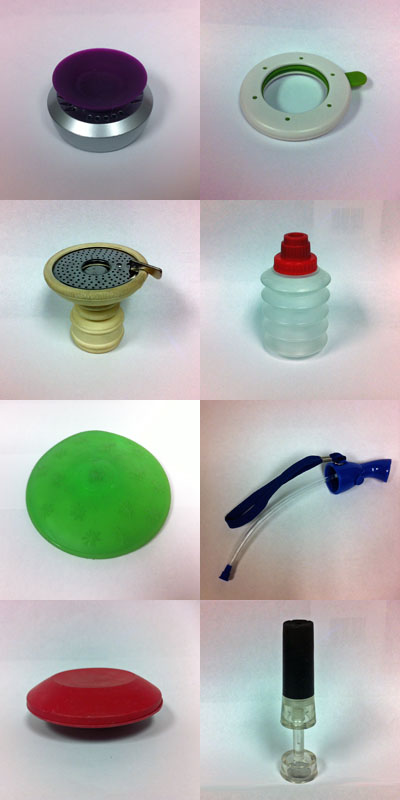
\includegraphics[width=2.5in]{figures/discourse_toys_images.jpg} 

    \caption{\label{fig:toys} The four pairs of toys used in Experiments 1A and 1B. Each toy had a unique affordance. First row: (left) the purple lid could be popped open and closed, and (right) the spaghetti sizer could be irised open and shut.  Second row: (left) the switch on the faucet aerator removed or revealed the center piece, and (right) the bottle could be squashed down and returned to size.  Third row: (left) the green disk was a squishy, malleable material, and (right) the tube was attached to a blue plastic piece with an inert button.  Fourth row: (left) the red top was bendable and could spin, and (right) the plastic section was clear and the top could be moved up and down. } 

  \end{center} 
\end{figure}

\section{Appendix B: Control Study}

We conducted a control study ruling out the possibility that response differences between Experiment 1A and 1B came from hearing 1 versus 2 comments before the naming event.  In the control, we ran an online version of our paradigm with 64 adults using Amazon's Mechanical Turk online crowd-sourcing service.  Participants responded to a single trial in one of two possible conditions: Embedded naming event between two comments (identical to Experiment 1A), or Embedded naming event after two comments and before one comment (so that the comments prior to the naming event were matched to Experiment 1B, but the comment following still qualified it as an Embedded trial here).  Naming location, toy order, and side were counterbalanced across participants. 

Results are plotted in Figure \ref{fig:control}. We found that adults were near ceiling in both naming conditions for selecting the first toy in First Toy trials (87\% after one comment and 94\% after two comments), and the second toy in Second Toy trials (100\% after one comment and 93\% after two comments).  These results suggest that participants' performance in Experiments 1A and 1B were not due to the number of comments they heard in a row, but rather to the naming event's location within a discourse structure.

\begin{figure}
  \begin{center} 
    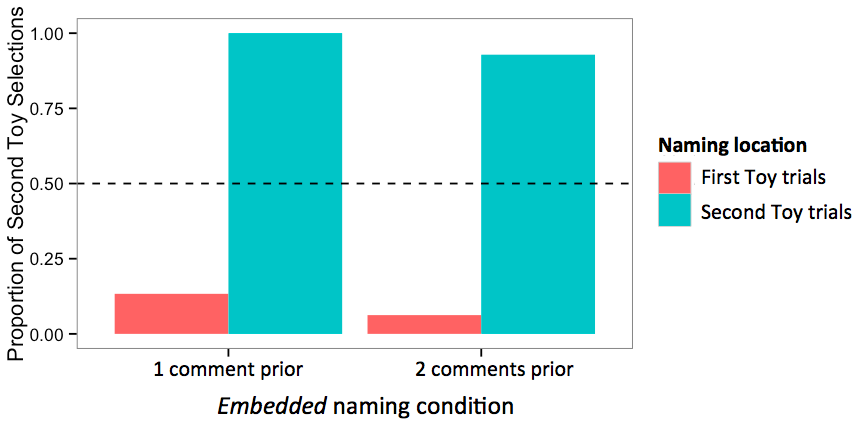
\includegraphics[width=5in]{figures/continuity_turk_2and3comments.png} 
    \caption{\label{fig:control} Results from Mechanical Turk control study manipulating the number of comments heard before the naming event, using the stimuli from Experiment 1B. Plotting conventions are as in Figure \ref{fig:res5}.} 
  \end{center} 
\end{figure}


% \begin{table}
%   \caption{Sample scripts for Experiments 1A and 1B across trial type (First Toy or Second Toy).  Naming location was counterbalanced across participants.  Red sentences are descriptions of the First Toy; blue sentences are descriptions of the Second Toy. Both were accompanied by unambiguous social cues. \label{tab:1b} } 
%   \begin{center} 
%   \small\addtolength{\tabcolsep}{-5pt}
%     \begin{tabular}{ll} 
%\scalebox{0.1}
%       \null   \textbf {Experiment 1A}  \\ 
%       \hline 
%       \textbf{Embedded First Toy} & \textbf{Embedded Second Toy} \\ 
%       \hline {\color{Red}The top of this one is wobbly.} &  {\color{Red} The top of this one is wobbly.} \\ 
%      \textbf{Have you seen a toma before?} &  {\color{Red} Look how to move this switch. }\\ 
%       {\color{Red}  Look how to move this switch.} & {\color{BlueGreen}The sides of this one are bumpy.}\\
%	  {\color{BlueGreen}The sides of this one are bumpy.} &   \textbf{Have you seen a toma before?} \\
%       {\color{BlueGreen}Look how to push the top down.} & {\color{BlueGreen} Look how to push the top down.} \bigskip \smallskip\\ 
%        \null    \textbf {Experiment 1B}  \\         
%       \hline 
%        \textbf{After First Toy} & \textbf{After Second Toy} \\ 
%       \hline {\color{Red}  The top of this one is wobbly.} & {\color{Red}The top of this one is wobbly.}\\ 
%      {\color{Red}Look how to move this switch.} & {\color{Red}Look how to move this switch. }\\ 
%  \textbf{Have you seen a toma before?} & {\color{BlueGreen} The sides of this one are bumpy.}\\
%       {\color{BlueGreen}The sides of this one are bumpy.}  & {\color{BlueGreen}  Look how to push the top down.}\\ 
%      {\color{BlueGreen}Look how to push the top down.} &   \textbf{Have you seen a toma before?} \\
%       \hline  \end{tabular} 
%   \end{center}
% \end{table}


\end{document}
